\documentclass[tikz,border=2pt]{standalone}

\usepackage[T1]{fontenc}
\usepackage{pgfplots}
\pgfplotsset{compat=1.18}

% Reconstructed from the exported figure because the raw plotting data/source is
% not present in the repository. Values are approximate digitizations from the
% image and are meant to provide an editable figure that can later be updated
% cleanly for CIC-IDS 2017 and CSE-CIC-IDS 2018.

\def\CICIDSRevisedX{9}
\def\CSECICIDSRevisedX{11}

\begin{document}
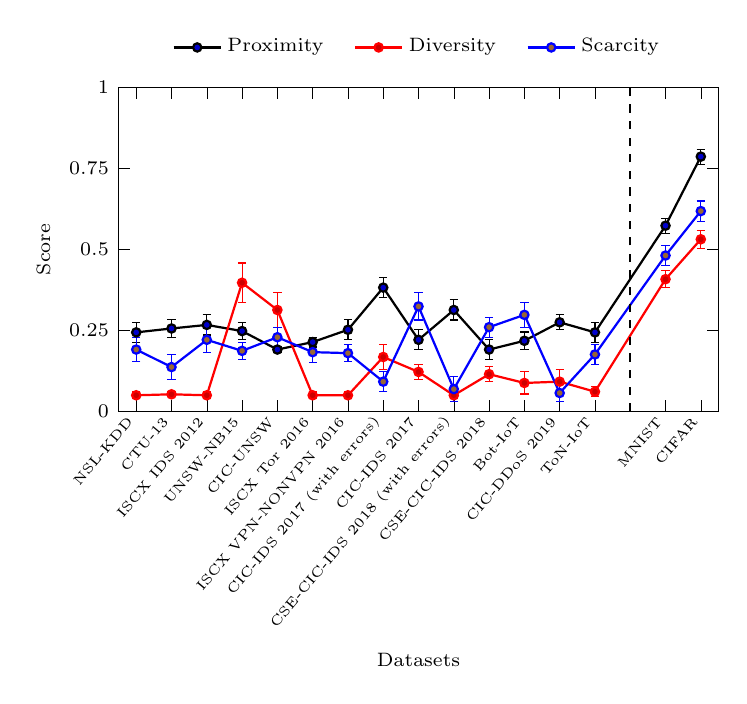
\begin{tikzpicture}
\begin{axis}[
    width=9.2cm,
    height=5.7cm,
    xmin=0.5,
    xmax=17.5,
    ymin=0,
    ymax=1,
    axis lines=box,
    xlabel={Datasets},
    ylabel={Score},
    xtick={1,2,3,4,5,6,7,8,9,10,11,12,13,14,16,17},
    xticklabels={
        NSL-KDD,
        CTU-13,
        ISCX IDS 2012,
        UNSW-NB15,
        CIC-UNSW,
        ISCX Tor 2016,
        ISCX VPN-NONVPN 2016,
        CIC-IDS 2017 (with errors),
        CIC-IDS 2017,
        CSE-CIC-IDS 2018 (with errors),
        CSE-CIC-IDS 2018,
        Bot-IoT,
        CIC-DDoS 2019,
        ToN-IoT,
        MNIST,
        CIFAR
    },
    ytick={0,0.25,0.5,0.75,1},
    xticklabel style={rotate=50,anchor=east,font=\tiny},
    yticklabel style={font=\scriptsize},
    xlabel style={font=\scriptsize},
    ylabel style={font=\scriptsize},
    tick style={black},
    legend style={
        at={(0.5,1.06)},
        anchor=south,
        legend columns=3,
        draw=none,
        font=\scriptsize,
        /tikz/every even column/.append style={column sep=0.9em}
    },
    clip=false,
]

\addplot+[black,thick,mark=*,mark size=1.5pt,error bars/.cd,y dir=both,y explicit]
coordinates {
    (1,0.244) +- (0,0.031)
    (2,0.256) +- (0,0.027)
    (3,0.267) +- (0,0.031)
    (4,0.248) +- (0,0.027)
    (5,0.191) +- (0,0.008)
    (6,0.214) +- (0,0.015)
    (7,0.252) +- (0,0.031)
    (8,0.382) +- (0,0.031)
    (9,0.221) +- (0,0.031)
    (10,0.313) +- (0,0.031)
    (11,0.191) +- (0,0.031)
    (12,0.218) +- (0,0.027)
    (13,0.275) +- (0,0.023)
    (14,0.244) +- (0,0.031)
    (16,0.573) +- (0,0.023)
    (17,0.786) +- (0,0.023)
};
\addlegendentry{Proximity}

\addplot+[red,thick,mark=*,mark size=1.5pt,error bars/.cd,y dir=both,y explicit]
coordinates {
    (1,0.050) +- (0,0.010)
    (2,0.053) +- (0,0.008)
    (3,0.050) +- (0,0.010)
    (4,0.397) +- (0,0.061)
    (5,0.313) +- (0,0.053)
    (6,0.050) +- (0,0.010)
    (7,0.050) +- (0,0.010)
    (8,0.168) +- (0,0.038)
    (9,0.122) +- (0,0.023)
    (10,0.050) +- (0,0.010)
    (11,0.115) +- (0,0.023)
    (12,0.088) +- (0,0.034)
    (13,0.092) +- (0,0.038)
    (14,0.061) +- (0,0.015)
    (16,0.408) +- (0,0.027)
    (17,0.531) +- (0,0.027)
};
\addlegendentry{Diversity}

\addplot+[blue,thick,mark=*,mark size=1.5pt,error bars/.cd,y dir=both,y explicit]
coordinates {
    (1,0.191) +- (0,0.038)
    (2,0.137) +- (0,0.038)
    (3,0.221) +- (0,0.038)
    (4,0.187) +- (0,0.027)
    (5,0.229) +- (0,0.031)
    (6,0.183) +- (0,0.031)
    (7,0.180) +- (0,0.027)
    (8,0.092) +- (0,0.031)
    (9,0.324) +- (0,0.042)
    (10,0.069) +- (0,0.038)
    (11,0.260) +- (0,0.031)
    (12,0.298) +- (0,0.038)
    (13,0.057) +- (0,0.027)
    (14,0.176) +- (0,0.031)
    (16,0.481) +- (0,0.031)
    (17,0.618) +- (0,0.031)
};
\addlegendentry{Scarcity}

\addplot[black,dashed,thick] coordinates {(15,0) (15,1)};

 % Later, revised values for CIC-IDS 2017 and CSE-CIC-IDS 2018 can be added by
 % overlaying a second marker style at x=\CICIDSRevisedX and x=\CSECICIDSRevisedX.
 % Example template:
 % \addplot+[only marks, mark=diamond*, red] coordinates {(\CICIDSRevisedX,0.18) (\CSECICIDSRevisedX,0.12)};

\end{axis}
\end{tikzpicture}
\end{document}
